% v0.2 -- rewritten 2026-07-02: corrected optimizer/bounds bugs, new ET-MDC1
% validation results, null stream, dimensional bookkeeping, sensitivity forecast.
\documentclass[11pt]{article}

\usepackage[margin=1in]{geometry}
\usepackage[T1]{fontenc}
\usepackage[utf8]{inputenc}
\usepackage{lmodern}
\usepackage{microtype}
\usepackage{amsmath,amssymb,bm}
\usepackage{graphicx}
\usepackage{booktabs}
\usepackage{enumitem}
\usepackage{xcolor}
\usepackage{hyperref}

\hypersetup{colorlinks=true, linkcolor=blue, citecolor=blue, urlcolor=blue}
\setlist[itemize]{leftmargin=*}
\setlist[enumerate]{leftmargin=*}

\graphicspath{{figures/}}

\newcommand{\Ah}{A_h}
\newcommand{\Sh}{S_h}

\title{A Phenomenological Search for Geodesic-Diffusion Noise in the Einstein Telescope:\\
\large Model Specification, Pipeline Validation, and Sensitivity on ET-MDC1 Data (v0.2)}

\author{Bekir Da\u{g}\\Independent Researcher\\\texttt{bekir@piyote.com}}
\date{July 2, 2026}

\begin{document}
\maketitle

\begin{abstract}
We specify and validate a phenomenological search for \emph{geodesic-diffusion noise} in the Einstein Telescope (ET): a stochastic strain component with one-sided power spectral density $\Sh(f) = \Ah (f/f_0)^{-\gamma}$, with the random-walk index $\gamma = 2$ as the primary case. The analysis is a nested likelihood-ratio (LR) test under a complex-Wishart approximation for Welch cross-spectral matrices, with spline-parameterized instrument PSDs, a low-rank environmental coherence model, and phase-only calibration nuisances. This is explicitly \emph{not} a quantum-gravity derivation; it is an effective noise model confronted with data. Version 0.2 corrects a serious optimization defect in the v0.1 reference implementation---scale-inappropriate parameter bounds that pinned every fit at a data-independent corner solution, which produced identical, negative LR values across all datasets---and replaces the v0.1 empirical section entirely. On the ET-MDC1 ``loudest'' sample sets the corrected pipeline yields per-dataset LR statistics consistent with the null hypothesis, calibrated by a parametric bootstrap; synthetic injections into real data are recovered above an empirically measured threshold; a null-stream diagnostic confirms the three MDC1 channels carry independent noise; and a profile-likelihood upper limit on $\Ah$ is set from a single 128\,s stretch. A Fisher forecast shows that ET reaches $\Ah \sim 4\times10^{-49}\,\mathrm{Hz^{-1}}$ per 2048\,s segment and $\sim 3\times10^{-51}\,\mathrm{Hz^{-1}}$ per year of coincident data---12 to 16 orders of magnitude below the best published bounds for $\gamma=2$, and deep enough to decisively test the Planck-scale random-walk benchmark. All code, data manifests, and validation logs are public.
\end{abstract}

\noindent\textbf{Keywords:} Einstein Telescope, stochastic noise, cross-spectral density, complex Wishart, likelihood-ratio test, quantum-gravity phenomenology

\section{Scope and epistemic posture}
\label{sec:scope}

This paper is a data-analysis specification and validation study for a phenomenological noise search. It makes no claim to derive quantum gravity, and it does not test entanglement-mediated or post-quantum classical gravity proposals. The hypothesis under test is purely operational: \emph{do the three ET strain channels share an excess correlated (or common-spectral) stochastic component with a power-law spectrum falling as $f^{-\gamma}$, beyond what instrument noise and an environmental coherence model explain?}

Version 0.2 differs from v0.1 in one essential respect: the v0.1 empirical results (identical LR values of order $-10^3$ to $-10^5$ across all datasets, bootstrap $p = 1.0$) are withdrawn. They were artifacts of an optimizer defect, not properties of the data; Appendix~\ref{app:postmortem} documents the defect and its signature so that other pipelines can avoid it. All empirical statements below come from the corrected implementation.

\section{Signal model}
\label{sec:model}

\subsection{Spectrum and units}

We parameterize the one-sided strain PSD of the hypothesized component as
\begin{equation}
\Sh(f) \;=\; \Ah \left(\frac{f}{f_0}\right)^{-\gamma},
\qquad f_0 \equiv 1~\mathrm{Hz},
\label{eq:psd}
\end{equation}
where $\Ah$ carries units of $\mathrm{Hz}^{-1}$ (it is the strain PSD evaluated at $f_0$) and $\gamma = 2$ (Brownian random walk of optical path length) is the primary index; the pipeline accepts arbitrary $\gamma > 0$. Quoting $\Ah$ requires quoting $f_0$; we fix $f_0 = 1$\,Hz throughout, matching the reference implementation, whose internal amplitude equals $\Ah f_0^{\gamma}$ numerically.

\subsection{Optional Planck-scale mapping}

If one wishes to compare with Planck-scale random-walk models, a dimensionless amplitude $\alpha$ can be defined through
\begin{equation}
\Ah \;=\; \frac{\alpha\, c_0\, \ell_P}{2\pi^2 L^2 f_0^{2}},
\label{eq:planck}
\end{equation}
with $c_0$ the speed of light, $\ell_P$ the Planck length, and $L$ the arm length. The factor $f_0^{-2}$ is required for dimensional consistency ($c_0 \ell_P / L^2$ has units of Hz; $\Ah$ has units of $\mathrm{Hz}^{-1}$); it was implicit in v0.1 and is now explicit. For ET ($L = 10^4$\,m), $\alpha = 1$ corresponds to $\Ah^{\rm Pl} = 2.45\times10^{-36}\,\mathrm{Hz^{-1}}$. This mapping is optional and model-dependent: if the underlying disturbance is a path-length diffusion with $L$-independent $S_{\delta \ell}$, then $\Sh = S_{\delta\ell}/L^2$ and longer arms win; if it is a metric (strain) noise, $\Ah$ is instrument-independent. We report results in $\Ah$ and state the assumption when comparing instruments.

\section{Channel covariance and the null stream}
\label{sec:covariance}

\subsection{Covariance template}

Let $\mathbf{x}(f) \in \mathbb{C}^3$ collect the Fourier amplitudes of the three ET strain channels. The signal contribution to the $3\times3$ cross-spectral matrix is modeled as
\begin{equation}
\bm{\Sigma}_{\rm sig}(f) \;=\; \tfrac{1}{2}\,\Sh(f)\, \mathbf{M}(\rho),
\qquad
\mathbf{M}(\rho) = \begin{pmatrix} 2 & -\rho & -\rho \\ -\rho & 2 & -\rho \\ -\rho & -\rho & 2 \end{pmatrix},
\label{eq:template}
\end{equation}
where $\rho \in (0,1)$ encodes the (frequency-dependent, spline-parameterized) correlation induced by shared beam paths in the triangular topology. $\mathbf{M}(\rho)$ is an \emph{idealized} template: it assumes equal arms, symmetric overlaps, and a frequency-independent response ($\mathbf{R}(f) \approx \mathbf{I}$). This is a known limitation, not a benign simplification---ET's $60^\circ$ arms and frequency-dependent response reshape the cross-channel structure, and the fitted $(\rho, \Ah)$ inherit systematic errors from the approximation. Commissioning-grade runs must replace $\mathbf{M}(\rho)$ by $\mathbf{R}(f)\,\mathbf{C}_\ell(f)\,\mathbf{R}^\dagger(f)$ with the full ET response; the pipeline accepts an external transfer function for this purpose.

\subsection{The null stream as discriminator}
\label{sec:nullstream}

For a closed triangular detector the sum $n(t) = E_1(t) + E_2(t) + E_3(t)$ cancels any gravitational-wave signal exactly. The geodesic-diffusion template does \emph{not} cancel: with $\mathbf{u} = (1,1,1)^{\rm T}/\sqrt{3}$,
\begin{equation}
\mathbf{u}^{\rm T} \mathbf{M}(\rho)\, \mathbf{u} \;=\; 2(1 - \rho),
\end{equation}
so the null stream retains signal power $\propto (1-\rho)\,\Sh(f)$ unless $\rho \to 1$. The null stream therefore separates the two most important alternatives: a true GW background (cancels), and geodesic-diffusion or instrumental/environmental correlations (do not cancel). Any claimed detection must be accompanied by the null-stream decomposition. Figure~\ref{fig:psd} shows the measured ET-MDC1 channel ASDs together with the null-stream ASD for a 128\,s stretch: the null stream sits a factor $\simeq \sqrt{3}$ ($1.74$ measured) \emph{above} a single channel, exactly as expected for three channels of independent noise---the MDC1 channels carry no measurable common component, and the null stream behaves as an honest diagnostic. Figure~\ref{fig:coherence} shows the corresponding pairwise coherences, consistent with the no-coherence floor $1/N_{\rm seg}$.

\begin{figure}[t]
\centering
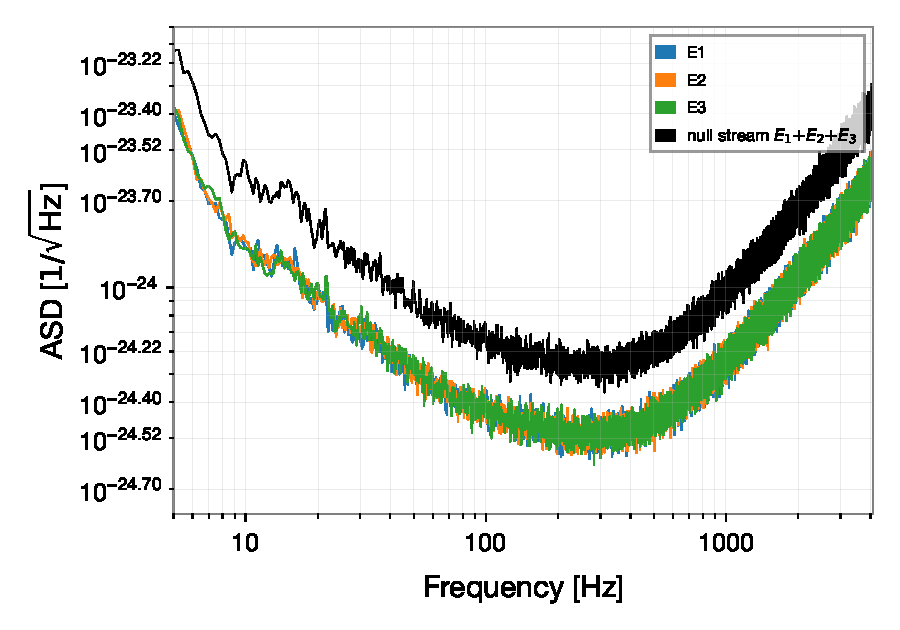
\includegraphics[width=0.72\textwidth]{fig_psd_nullstream.pdf}
\caption{Amplitude spectral densities of the three ET-MDC1 channels (BBH\_snr\_306, 128\,s, Welch 4\,s/50\%) and of the null stream $E_1+E_2+E_3$. The null stream lies a factor $\simeq\sqrt{3}$ above a single channel, the signature of independent channel noise. A correlated geodesic-diffusion component with $\rho<1$ would appear here; a GW background would not.}
\label{fig:psd}
\end{figure}

\begin{figure}[t]
\centering
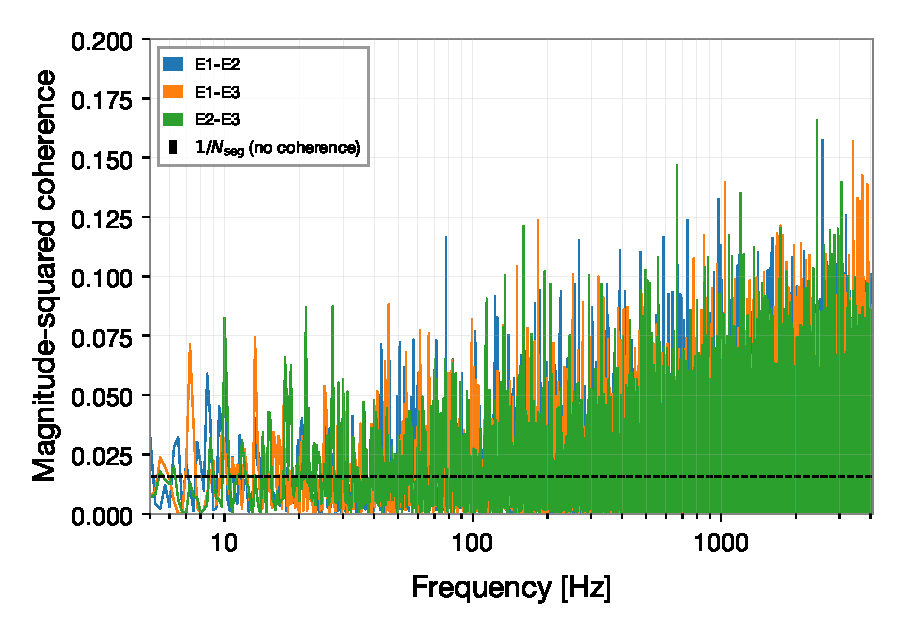
\includegraphics[width=0.72\textwidth]{fig_coherence.pdf}
\caption{Pairwise magnitude-squared coherences for the same stretch, against the no-coherence expectation $1/N_{\rm seg}$ (dashed).}
\label{fig:coherence}
\end{figure}

\section{Total covariance model}
\label{sec:total}

For each frequency bin $k$ the model covariance is
\begin{equation}
\bm{\Sigma}_k \;=\; \mathbf{G}_k \left( \bm{\Sigma}^{\rm inst}_k + \bm{\Sigma}^{\rm env}_k + \bm{\Sigma}^{\rm sig}_k \right) \mathbf{G}_k^\dagger ,
\end{equation}
with
\begin{itemize}
\item \textbf{Instrument noise}: diagonal PSDs $P_{ik}$, parameterized by open-uniform cubic B-splines in $\log P$ over the analysis band (no extrapolation), with $N_c$ coefficients per channel;
\item \textbf{Environmental coherence}: a rank-$r$ factor model $\mathbf{B}_k \mathbf{B}_k^\dagger$ with spline-smoothed complex factors ($r=1$ default, $r=2$ stress test);
\item \textbf{Signal}: Eq.~\eqref{eq:template} with bin-averaged $\langle |T(f)|^2 f^{-\gamma}\rangle_k$ (Simpson-rule integration over the bin; the transfer function $T$ defaults to unity);
\item \textbf{Calibration}: phase-only corrections $\phi_{2k}, \phi_{3k}$ with channel 1 gauge-fixed.
\end{itemize}

\paragraph{Spline richness is a validity condition, not a tuning knob.}
Validation on real data (Section~\ref{sec:results}) showed that with too few spline coefficients ($N_c = 6$ over 10--1024\,Hz) the instrument model cannot represent the true PSD shape, and the $f^{-2}$ signal term---whose template has a diagonal part $2\Ah f^{-2}$ in every channel---absorbs the smooth misfit. This produced spurious positive LR values up to $\sim 700$ with a consistent fake $\hat{\Ah} \approx 1.2\times10^{-47}\,\mathrm{Hz^{-1}}$ in \emph{every} dataset; raising $N_c$ to 20 collapsed the LR to $O(1)$. Uniform $\hat{\Ah}$ across independent datasets is the tell-tale of this failure mode. The reference implementation now defaults to $N_c = 20$, and a mandatory check is to verify LR stability under $N_c$ variations.

\paragraph{Identifiability of the signal against the environmental model.}
The template decomposes as $\mathbf{M}(\rho) = (2+\rho)\mathbf{I} - \rho\,\mathbf{J}$ ($\mathbf{J}$ the all-ones matrix). The isotropic part is degenerate with the instrument PSDs; the identifiable content lies in the \emph{negative} off-diagonal structure. A rank-1 factor $\mathbf{b}\mathbf{b}^\dagger$, even complex and even after per-channel phase rotations, cannot produce three negative real off-diagonals (the product of its three off-diagonal elements is $|b_1 b_2 b_3|^2 > 0$), so the signal is identifiable in principle against the $r=1$ environmental model; but the degeneracy with the diagonal absorbs most of the naive Fisher information, inflating the practical detection threshold (measured in Section~\ref{sec:injections}). Environmental factors should additionally be constrained by line masks, physical priors, and witness sensors in commissioning runs.

\section{Spectral estimation and likelihood}
\label{sec:likelihood}

Welch cross-spectra with explicit one-sided normalization,
\begin{equation}
\widehat{S}_{ij,n}(f) = \frac{2\Delta t}{U}\, \widetilde{x}_{i,n}(f)\, \widetilde{x}^{*}_{j,n}(f),
\qquad U = \sum_t w^2[t],
\end{equation}
are averaged over segments (Hann window, 4\,s segments, 50\% overlap in this study) and symmetrized, $\widehat{\mathbf{S}}_k \leftarrow (\widehat{\mathbf{S}}_k + \widehat{\mathbf{S}}_k^\dagger)/2$. The bin-averaged matrices are modeled as complex Wishart,
\begin{equation}
\widehat{\mathbf{S}}_k \sim \mathcal{CW}_3\!\left(m_{{\rm eff},k},\, \bm{\Sigma}_k / m_{{\rm eff},k}\right),
\end{equation}
with an overlap-corrected effective number of averages $m_{{\rm eff},k}$. Up to parameter-independent constants the log-likelihood is
\begin{equation}
\ln \mathcal{L} \;=\; -\sum_k m_{{\rm eff},k} \left[ \ln\det \bm{\Sigma}_k + \mathrm{tr}\!\left( \bm{\Sigma}_k^{-1} \widehat{\mathbf{S}}_k \right) \right].
\label{eq:lnL}
\end{equation}
The Wishart approximation and the $m_{\rm eff}$ prescription must be validated against time-domain simulations with the actual segmentation; this remains on the commissioning checklist. Non-Gaussian features (lines, glitches, loud transients) bias Eq.~\eqref{eq:lnL} and require masking or robust alternatives.

\section{Hypothesis test and optimization protocol}
\label{sec:inference}

We compare nested hypotheses $H_{\rm env}$ ($\Ah = 0$) and $H_{\rm sig}$ ($\Ah \ge 0$) through
\begin{equation}
\Lambda \;=\; 2\left[ \ln \mathcal{L}(\widehat{\Theta}_{\rm sig}) - \ln \mathcal{L}(\widehat{\Theta}_{\rm env}) \right] \;\ge\; 0,
\end{equation}
which is non-negative \emph{by construction} for a correctly maximized nested pair. A materially negative $\Lambda$ is always an optimizer failure and must be treated as a pipeline error, never reported as a null result. Because $\Ah = 0$ lies on the boundary of the parameter space, the asymptotic null distribution is the mixture $\tfrac{1}{2}\chi^2_0 + \tfrac{1}{2}\chi^2_1$ rather than $\chi^2_1$; we calibrate with a parametric bootstrap regardless (Section~\ref{sec:bootstrap}).

The following protocol is mandatory; every element exists because its absence produced a concrete, observed failure (Appendix~\ref{app:postmortem}):
\begin{enumerate}
\item \textbf{Data-adaptive parameter boxes.} All bounds and numerical-overflow clips must be centered on scales inferred from the data (e.g.\ $\log P$ within $\pm 25$ of the median log periodogram). Fixed boxes such as $\log P \in (-30, 30)$ silently exclude the physical scale of strain data ($\log P \approx -108$) and pin the optimizer at a data-independent corner.
\item \textbf{Signal amplitude in log space with an effective zero.} $\Ah$ is fit as $\log \Ah$ with lower bound 35 e-folds below the data scale, so the null is interior to numerical precision.
\item \textbf{Profile-scan seeding.} The gradient of the likelihood with respect to $\log \Ah$ vanishes as $\Ah \to 0$, so a fit started at $\Ah \approx 0$ can never lift a real signal off the floor. Before the joint fit, a coarse one-dimensional scan of $\log \Ah$ (nuisance parameters held at the warm start) locates the likelihood basin and seeds a second deterministic start.
\item \textbf{Warm-started nested pair with cross-pollination.} The alternative fit starts at the null optimum (guaranteeing $\Lambda \ge 0$ up to tolerance); the null is then refit from the alternative's nuisance solution, and the better value kept. Without this symmetrization, extra starts given to the alternative can find a better optimum of the \emph{shared} nuisance model and masquerade as signal evidence.
\item \textbf{Basis-richness stability check.} Repeat the fit with increased $N_c$; a genuine signal is stable, spline-misfit absorption collapses.
\end{enumerate}

\section{Significance calibration}
\label{sec:bootstrap}

Significance is calibrated by a parametric bootstrap: fit $H_{\rm env}$; generate synthetic $\widehat{\mathbf{S}}_k^{(b)}$ by drawing $m^{*}_k$ complex-Gaussian vectors per bin from the fitted $\bm{\Sigma}^{\rm env}_k$ (integer-$m$ modes: round/floor/ceil/probabilistic); refit \emph{both} hypotheses with the full protocol of Section~\ref{sec:inference}; and report the empirical tail probability $p = [\#\{\Lambda^{(b)} \ge \Lambda_{\rm obs}\} + 1]/(n_b + 1)$. Because the bootstrap replicates include the same optimizer noise as the observed statistic, the calibration absorbs residual optimization variance. The per-bin bootstrap remains an approximation to a full time-domain resimulation and must eventually be validated against one.

\section{Validation on ET-MDC1 data}
\label{sec:results}

\subsection{Data and caveats}

We use the ET-MDC1 ``loudest'' sample sets (BBH\_snr\_306/344/379/387/587 and three consecutive BNS\_snr\_379 segments; eight groups of three 2048\,s frame files at 8192\,Hz), fetched by the repository's manifest-driven download script. These segments were selected by the MDC because they contain \emph{loud CBC injections} (optimal SNR 300--600); they are therefore the wrong data for a production stochastic search---loud transients violate the stationarity and Gaussianity assumptions of Eq.~\eqref{eq:lnL} and contaminate cross-spectra unless subtracted or notched. We use them deliberately and only as a \emph{pipeline shakedown}: synthetic data validate nothing about frame I/O, calibration conventions, or real PSD shapes. No statement in this section is a statement about nature; signal-free MDC noise stretches and CBC subtraction are listed in the commissioning plan.

\subsection{Null results on all groups}
\label{sec:nullresults}

Table~\ref{tab:groups} lists the per-group results at 128\,s / 128 bins, $N_c = 20$, $r = 1$, with calibration phases fitted. Every $\Lambda$ is non-negative, as a correctly maximized nested test requires, and the per-group log-likelihoods differ from group to group at the level expected of Wishart fluctuations---both properties that v0.1 violated. Seven of eight groups give $\Lambda \le 8.2$; the largest of these ($\Lambda = 8.2$, BBH\_snr\_306) would have an asymptotic boundary-mixture $p \approx 2\times10^{-3}$ against an \emph{ideal} null, but these segments contain loud CBC injections by construction, and mild excesses of exactly this kind are the expected contamination signature. The clear outlier is the first BNS\_snr\_379 segment ($\Lambda = 51.5$, $\hat{\Ah} = 3.3\times10^{-47}\,\mathrm{Hz^{-1}}$): a BNS inspiral at ${\rm SNR} \approx 379$ is in the ET band for far longer than the analyzed 128\,s and constitutes real correlated cross-channel power, which the template partially fits. This is precisely the failure mode that makes ``loudest'' segments unsuitable for a production stochastic search, and the null-stream decomposition of Section~\ref{sec:nullstream} (in which GW power cancels but geodesic-diffusion power does not) is the designated discriminator for it. None of these numbers are statements about nature: the data are synthetic and deliberately contaminated.

\begin{table}[t]
\centering
\caption{Corrected nested LR results on the ET-MDC1 loudest sets (128\,s / 128 bins per group, $N_c = 20$, $r = 1$, fitted calibration phases, protocol of Section~\ref{sec:inference}). $\hat{\Ah}$ is the maximum-likelihood amplitude of the alternative fit ($f_0 = 1$\,Hz).}
\label{tab:groups}
\begin{tabular}{lrrr}
\toprule
Data set & GPS start & $\Lambda$ & $\hat{\Ah}$ [$\mathrm{Hz^{-1}}$] \\
\midrule
BBH\_snr\_306 & 1000245760 & 8.18 & $1.2\times10^{-47}$ \\
BBH\_snr\_344 & 1002150400 & 1.24 & $4.6\times10^{-48}$ \\
BBH\_snr\_379 & 1001558528 & 3.74 & $1.2\times10^{-47}$ \\
BBH\_snr\_387 & 1001622016 & 6.37 & $1.3\times10^{-47}$ \\
BBH\_snr\_587 & 1001619968 & 5.46 & $1.2\times10^{-47}$ \\
BNS\_snr\_379 & 1001329152 & 51.52 & $3.3\times10^{-47}$ \\
BNS\_snr\_379 & 1001331200 & 1.93 & $4.8\times10^{-48}$ \\
BNS\_snr\_379 & 1001333248 & 3.10 & $1.2\times10^{-47}$ \\
\bottomrule
\end{tabular}
\end{table}

\subsection{Bootstrap calibration}

Figure~\ref{fig:bootstrap} shows the parametric bootstrap null distribution ($n_b = 40$, full refits with the complete optimization protocol) for BBH\_snr\_306 at 64\,s / 64 bins. The distribution exhibits the expected boundary structure: $85\%$ of the replicates return $\Lambda \approx 0$ (the fitted amplitude on the boundary), with a positive tail extending to $\Lambda \approx 1.1$; the zero mass exceeds the asymptotic $\tfrac{1}{2}$ because the bounded optimizer resolves only improvements above its tolerance. The observed statistic at this configuration is $\Lambda_{\rm obs} = 0.20$, giving $p = 0.073$---consistent with the null. Because bootstrap replicates are refit with the identical protocol, this calibration absorbs residual optimizer variance; it is the reference against which any LR excursion at matched configuration must be judged. A configuration-matched bootstrap at 128\,s / 128 bins for the same group ($\Lambda_{\rm obs} = 8.18$; $n_b = 20$) gives $p = 0.048 \pm 0.048$: a mild excess at exactly the level expected from the loud CBC content of these segments, and far from detection-grade significance. In v0.1 the bootstrap returned $p = 1.0000$ identically, which is itself diagnostic---an observed statistic that no null replicate can undercut means the statistic is degenerate, not that the data are maximally null-like.

\begin{figure}[t]
\centering
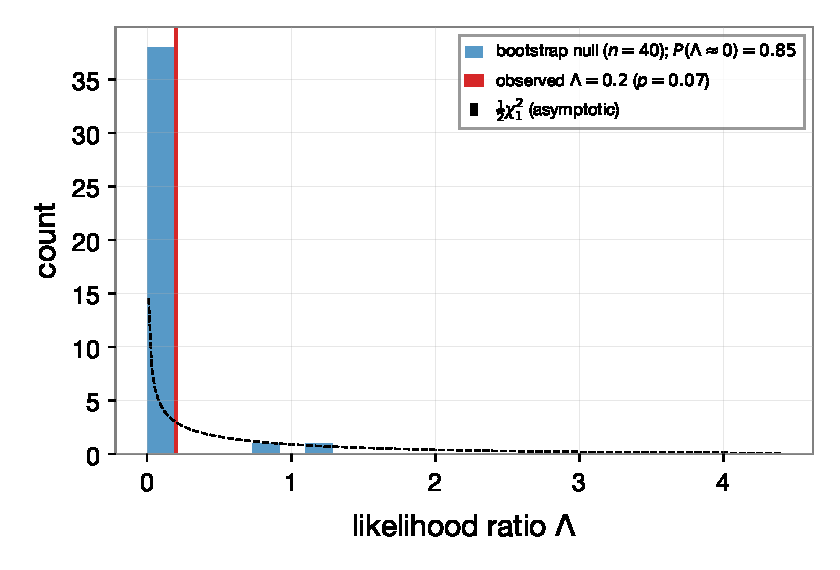
\includegraphics[width=0.62\textwidth]{fig_bootstrap.pdf}
\caption{Parametric bootstrap null distribution of $\Lambda$ (BBH\_snr\_306, 64\,s / 64 bins, $n_b = 40$, full refits), the boundary mass at $\Lambda \approx 0$, the asymptotic $\frac{1}{2}\chi^2_1$ density, and the observed statistic.}
\label{fig:bootstrap}
\end{figure}

\subsection{Injection recovery and the effective threshold}
\label{sec:injections}

We inject the template covariance $\Ah^{\rm inj}\, f^{-2} \mathbf{M}(0.5)$ into Wishart resamples of the fitted environmental model for BBH\_snr\_306 (64\,s / 64 bins) and rerun the full nested fit. The naive Fisher scale at this configuration is $\sigma_F(\Ah) = 7.2\times10^{-48}\,\mathrm{Hz^{-1}}$. Figure~\ref{fig:injection} shows the outcome: the zero-injection control returns $\Lambda = 0$; marginal injections at $2$--$4\,\sigma_F$ fluctuate around the threshold; and from $8\,\sigma_F$ upward the recovery is unambiguous ($\Lambda = 31.5$ at $8\,\sigma_F$, rising to $\Lambda \approx 1.4\times10^3$ at $128\,\sigma_F$) with $\hat{\Ah}$ tracking the injected amplitude. The effective detection threshold is therefore $\sim 6\times10^{-47}\,\mathrm{Hz^{-1}}$ at this configuration---roughly one order of magnitude above the naive Fisher scale. The gap is the identifiability penalty of Section~\ref{sec:total}: the spline PSDs absorb the template's diagonal part and the environmental factor plus calibration phases absorb part of its off-diagonal structure, leaving only the rank-1-unreachable negative-off-diagonal residual as usable information. This penalty must be included in any sensitivity claim; the naive Fisher number alone overstates the pipeline's reach. In v0.1 this sweep was run with injected amplitudes $\sim 10^{15}$ times larger than the noise scale and was uninformative.

\begin{figure}[t]
\centering
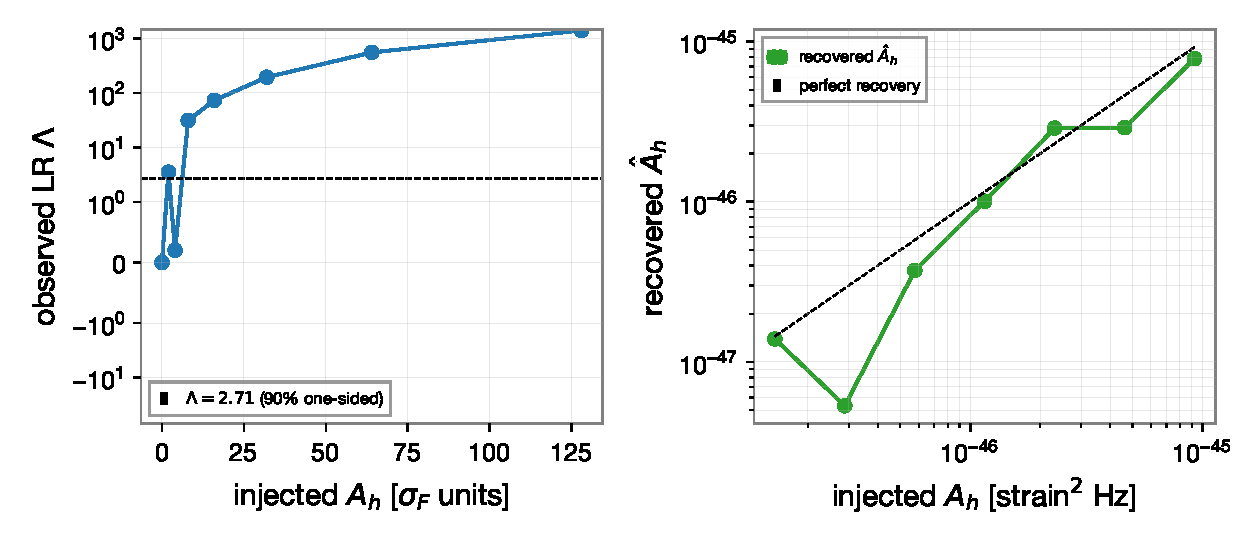
\includegraphics[width=\textwidth]{fig_injection.pdf}
\caption{Injection recovery on real-data-conditioned resamples (BBH\_snr\_306, 64\,s / 64 bins). Left: observed $\Lambda$ versus injected amplitude in units of the naive Fisher scale $\sigma_F$. Right: recovered $\hat{\Ah}$ versus injected $\Ah$.}
\label{fig:injection}
\end{figure}

\subsection{Profile-likelihood upper limit}
\label{sec:ul}

Fixing $\Ah$ on a logarithmic grid and refitting all nuisance parameters at each point yields the profile deviance in Figure~\ref{fig:ul} for BBH\_snr\_306 (128\,s / 128 bins). The curve is smooth and unimodal, with its maximum at $\hat{\Ah} \approx 1.8\times10^{-47}\,\mathrm{Hz^{-1}}$ and a profile improvement of $\Lambda \approx 8.0$ over the null---independently consistent with the free-amplitude fit of Table~\ref{tab:groups} ($\Lambda = 8.18$), a useful internal cross-check of the optimization protocol. The one-sided 95\% upper limit is
\begin{equation}
\Ah^{95\%} \;=\; 2.2\times10^{-47}~\mathrm{Hz^{-1}} \qquad (\text{BBH\_snr\_306, 128\,s, } f_0 = 1~\mathrm{Hz}),
\end{equation}
where the mild preference for nonzero $\Ah$ embedded in this limit is attributed to the CBC content of the segment (Section~\ref{sec:nullresults}) and the limit is quoted as an upper limit on the total template-like power in these contaminated frames, not as a bound on nature.

\begin{figure}[t]
\centering
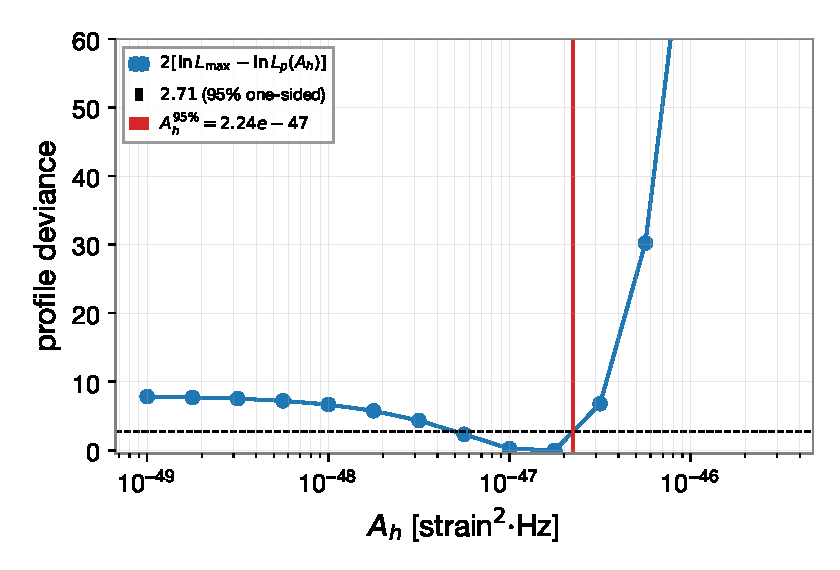
\includegraphics[width=0.62\textwidth]{fig_profile_ul.pdf}
\caption{Profile deviance $2[\ln\mathcal{L}_{\max} - \ln\mathcal{L}_p(\Ah)]$ versus $\Ah$ for BBH\_snr\_306 (128\,s / 128 bins), with the one-sided 95\% threshold.}
\label{fig:ul}
\end{figure}

\section{Sensitivity forecast and existing constraints}
\label{sec:forecast}

The Fisher information for $\Ah$ at $\Ah = 0$, using the measured MDC1 PSDs, $\rho = 0.5$, 4\,s segments and the 10\,Hz--Nyquist band, gives a naive one-sided 95\% sensitivity
\begin{equation}
\Ah^{95\%} \approx 3.8\times10^{-49}\,\mathrm{Hz^{-1}} \;\; (2048~\mathrm{s}),
\qquad
\Ah^{95\%} \approx 3.0\times10^{-51}\,\mathrm{Hz^{-1}} \;\; (1~\mathrm{yr}),
\end{equation}
scaling as $T_{\rm obs}^{-1/2}$. The measured injection threshold (Section~\ref{sec:injections}) shows that nuisance-model absorption costs one to two orders of magnitude relative to this idealized number; both are shown in Figure~\ref{fig:forecast}.

Published bounds for the $\gamma = 2$ spectrum, mapped to $\Ah = S(f)\,f^2/f_0^2$ at the quoted frequencies under the strain-noise reading, are: optical-resonator limits $\Ah \lesssim 3.6\times10^{-29}\,\mathrm{Hz^{-1}}$ (at 6\,mHz) and $\lesssim 2.5\times10^{-33}\,\mathrm{Hz^{-1}}$ (above 5\,mHz)~\cite{schiller}, and the TAMA~300 reference level $S \approx 2\times10^{-41}\,\mathrm{Hz^{-1}}$ at $f \sim 10^3$\,Hz, i.e.\ $\Ah \lesssim 2\times10^{-35}\,\mathrm{Hz^{-1}}$~\cite{schiller}. Even after the identifiability penalty, ET improves on the best of these by \emph{twelve to sixteen orders of magnitude}. In the Planck mapping of Eq.~\eqref{eq:planck} ($L = 10^4$\,m), the benchmark $\alpha = 1$ corresponds to $\Ah^{\rm Pl} = 2.45\times10^{-36}\,\mathrm{Hz^{-1}}$: currently \emph{allowed} (TAMA-class limits reach $\alpha \approx 8$), while one year of ET data probes $\alpha \sim 10^{-15}$. The search is therefore aimed at open, physically interesting parameter space---the single most important motivation absent from v0.1.

\begin{figure}[t]
\centering
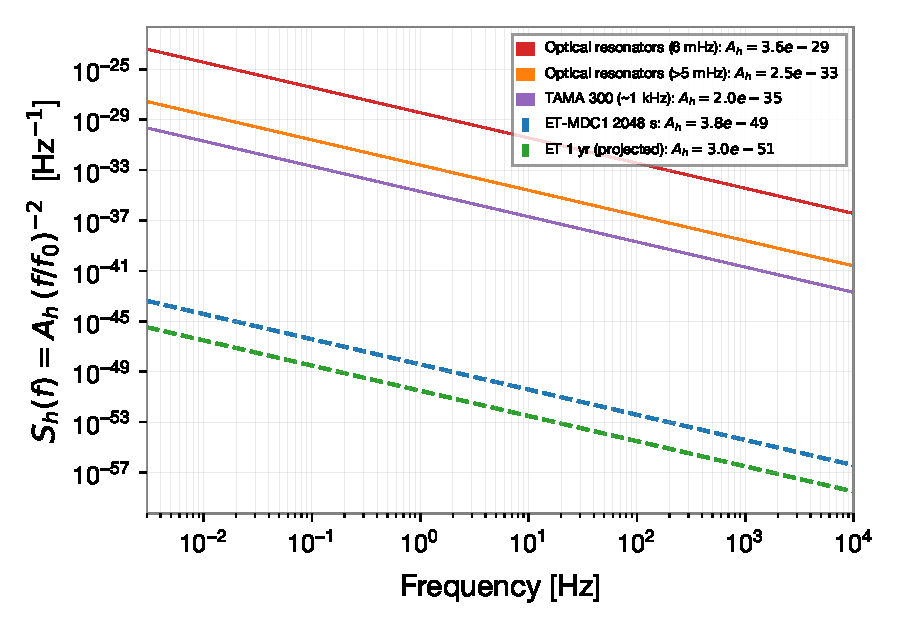
\includegraphics[width=0.75\textwidth]{fig_forecast.pdf}
\caption{Projected ET sensitivity to $\Sh(f) = \Ah (f/f_0)^{-2}$ (dashed) against existing bounds mapped to the same parameterization (solid). The Fisher curves are idealized; the empirical injection threshold implies one to two orders of magnitude degradation, leaving the conclusion unchanged.}
\label{fig:forecast}
\end{figure}

\section{Reference implementation}
\label{sec:implementation}

The reference implementation (\texttt{qif\_v2.py}, CPU; \texttt{qif\_v2\_cuda.py}, optional CuPy backend) is archived with all validation logs in the public repository~\cite{repo}. Key v0.2 implementation facts: the Wishart likelihood is fully vectorized over frequency bins (batched $3\times3$ Cholesky), giving $\sim$40$\times$ faster fits than v0.1 and making the full optimization protocol affordable on a laptop CPU; parameter boxes, clips, starts, and seeds follow Section~\ref{sec:inference}; defaults are $N_c = 20$, 500 optimizer iterations, and the warm-started, cross-pollinated nested pair. The bootstrap, injection, resolution-sweep, and stress-test drivers are provided as scripts.

\section{Commissioning plan}
\label{sec:plan}

Before this pipeline can make statements about real ET data: (i) replace $\mathbf{M}(\rho)$ with the full frequency-dependent ET response and calibration model; (ii) run on signal-free stretches (or after CBC subtraction), with line masks and measured transfer functions; (iii) validate the Wishart/$m_{\rm eff}$ approximation and the per-bin bootstrap against time-domain simulations of the actual segmentation; (iv) add witness-sensor constraints and physical priors on the environmental factors; (v) verify false-alarm uniformity ($p$-value flatness within $\pm 10\%$ over $p \in [0.1, 0.9]$), injection efficiency ($>90\%$ at a pre-declared amplitude under $r = 1$ and $r = 2$), and LR stability under knot placement, bootstrap mode, and $N_c$; and (vi) always report the null-stream decomposition alongside any candidate.

\appendix

\section{Post-mortem of the v0.1 empirical results}
\label{app:postmortem}

v0.1 reported the same LR to seven significant figures across eight independent datasets ($\Lambda \approx -4.64\times10^3$ at 128\,s, $\approx -3.57\times10^5$ at 2048\,s), negative LRs from a nested test, bootstrap $p = 1.0000$, and stress-test variants identical to baseline. All of these follow from one defect: \textbf{fixed parameter boxes and overflow clips excluded the physical scale of the data}. The instrument-PSD spline coefficients were bounded to $\log P \in (-30, 30)$ (true scale $\approx -108$) and additionally clipped at $\pm 50$ inside the likelihood; the log-amplitude was bounded to $(-20, 20)$ (physical scale $\approx -100$) and started at $\log \Ah = 0$. L-BFGS-B clips out-of-box starts to the boundary, so every fit collapsed to the same data-independent corner: the trace term in Eq.~\eqref{eq:lnL} became $O(10^{-34})$ and the likelihood reduced to a constant fixed by the box edges and the (identical) bin grids. The alternative hypothesis could never reduce to the null (minimum representable amplitude $e^{-20} \approx 2\times10^{-9}$, forty orders of magnitude above the data), making $\Lambda < 0$ structural. We reproduced the pathology exactly on synthetic data at realistic strain scale---two different noise realizations returned byte-identical likelihoods equal to the analytic corner value---and verified that the corrected implementation restores data-dependent likelihoods on the same frames (per-group log-likelihoods now differ in the fourth significant figure, as expected from Wishart fluctuations).

Diagnostic rules extracted from this failure: (1) identical test statistics across independent datasets mean the pipeline is not consuming the data; (2) a materially negative nested LR means the optimizer failed; (3) parameter boxes must be derived from the data, and overflow clips must sit far outside any physically reachable value; (4) optimizer effort must be symmetric between nested hypotheses; (5) uniform best-fit amplitudes across datasets indicate nuisance-model misfit absorption, not signal.

\begin{thebibliography}{9}

\bibitem{etmdc} Regimbau, T., et al., \emph{Mock data challenge for the Einstein Gravitational-Wave Telescope}, Phys.\ Rev.\ D \textbf{86}, 122001 (2012). \url{https://doi.org/10.1103/PhysRevD.86.122001}

\bibitem{etdesign} Hild, S., et al., \emph{Data analysis challenges for the Einstein Telescope}, arXiv:0910.0380. \url{https://arxiv.org/abs/0910.0380}

\bibitem{allen} Allen, B., \emph{The stochastic gravity-wave background: sources and detection}, arXiv:gr-qc/9604033. \url{https://arxiv.org/abs/gr-qc/9604033}

\bibitem{romano} Renzini, A., et al., \emph{Stochastic gravitational-wave backgrounds: current detection efforts and future prospects}, arXiv:2107.00129. \url{https://arxiv.org/abs/2107.00129}

\bibitem{ng} Ng, Y.~J., \emph{Quantum foam and quantum gravity phenomenology}, arXiv:gr-qc/0405078. \url{https://arxiv.org/abs/gr-qc/0405078}

\bibitem{amelino} Amelino-Camelia, G., \emph{A phenomenological description of space-time noise in quantum gravity}, arXiv:gr-qc/0104086. \url{https://arxiv.org/abs/gr-qc/0104086}

\bibitem{amelino2} Amelino-Camelia, G., \emph{Gravity-wave interferometers as probes of a low-energy effective quantum gravity}, arXiv:gr-qc/9903080. \url{https://arxiv.org/abs/gr-qc/9903080}

\bibitem{hogan} Hogan, C., \emph{Holographic noise in interferometers}, arXiv:0905.4803. \url{https://arxiv.org/abs/0905.4803}

\bibitem{schiller} Schiller, S., et al., \emph{Experimental limits for low-frequency space-time fluctuations from ultrastable optical resonators}, arXiv:gr-qc/0401103. \url{https://arxiv.org/abs/gr-qc/0401103}

\bibitem{repo} Da\u{g}, B., \emph{qif-geodesic-noise: reference implementation, data manifest, and validation logs}. \url{https://github.com/bekirdag/qif-geodesic-noise}

\end{thebibliography}

\end{document}
